\documentclass{article}
\usepackage{graphicx}
\usepackage[section]{placeins}
\usepackage{hyperref}
\usepackage{algorithm}
\usepackage[noend]{algpseudocode}
\usepackage{dirtree}
\usepackage{amsfonts}
\usepackage{amsmath}

\algnewcommand\algorithmicassert{\texttt{assert}}
\algnewcommand\Assert[1]{\State \algorithmicassert(#1)}%



\makeatletter
\def\BState{\State\hskip-\ALG@thistlm}
\makeatother


\begin{document}
{\huge \textbf{Agradecimientos}}\\
\\
A los profesores.\\
A mi familia.\\
A mi novia y su familia.\\
A mis amigos de la Vieja Escuela.\\
A FaMAF de punta a punta.\\
A mis amigos de Ascentio.\\
A mis amigos la Bicicleta.\\ 
A Dios que es grande.\\
\\
En memoria de mis abuelos que tambi\'en dieron sus pasos por la UNC.\\\\
\noindent
Por su paciencia.\\
Por su perseverancia.\\
Por su temple.\\
Por los valores.\\
\\
Muchas Gracias!


\newpage
\section{Marco de trabajo e investigacion}

En el proceso de investigacion del fenomeno fisico de Resonancia Magnetica Nuclear el investigador manipula modulos 
electronicos digitales de medicion precisos, estables y en algunos casos si intervienen mas de uno a la vez entre ellos sincronizados 
por medio de interfaces digitales. Estos modulos electronicos digitales colaboran con la creacion del contexto necesario para investigar lo planeado 
segun la necesidad del investigador. En general junto con los modulos electronicos intervienen otros modulos electronicos de naturaleza analogica
tales como amplificadores operacionales, mezcladores de señales, filtros pasa bajos entre otros.

La correcta conexion entre los diferentes modulos electronicos digitales, analogicos y su configuracion durante el proceso de experimentacion
son responsabilidad del investigador y una tarea de suma importancia para el exito de la experiencia a realizar.

En este marco de responsabilidades del investigador y el modulo digital a ser utilizado es deseable y necesaria mecanismos sencillos de manipulacion
del mismo y su monitoreo.

\subsection{Rol del Software}

El rol primario del software en el contexto descripto previamente es el de manipular el modulo digital a traves de la PC utilizada por el investigador 
de forma local o remota.

El rol secundario la administracion de usuarios del modulo digital, monitoreo de los experimentos en curso y resultados.


\section{Partes de un experimento}

Estos son algunos conceptos clave para comprender el contexto y definici\'on de un
experimento, los cuales se tuvieron en cuenta al momento de la implementaci\'on 
del sistema.

\subsubsection{Pulso de radio frecuencia}
Es una se\~nal senoidal que tiene como objetivo
estimular la muestra presente en el resonador
y que puede ser manipulada previamente
por otros m\'odulos externos. Tiene los siguientes atributos:
    \begin{itemize}
        \item Frecuencia: 0 a 120 megahercios.
        \item Fase: 0 a 360 grados.
        \item Duraci\'on: 0 a 16 segundos.
    \end{itemize}

\subsubsection{Pulso TTL}
Es una se\~nal digital de amplitud 5V y duraci\'on predefinida con la finalidad de trasmitirla como entrada a otros m\'odulos digitales o anal\'ogicos para sicronizar momentos de relajaci\'on y estimulaci\'on de las muestras durante la experiencia.

\subsubsection{Muestras}
Las muestras son un grupo de datos obtenidos a cierta frecuenta de muestreo y agrupados de manera contigua 
en un bloque de longitud $2^{n}$ con $n \in \mathbb{N}$. 

\subsection{Tipo de Experiencia}
El tipo de experiencia a realizar esta determinada por el investigador, existen 2 bien difrenciadas:

\subsubsection{Experiencia Promedio}
Una experiencia promedio es una que se repite y donde los bloques de muestras ordenadas se suman uno a uno obteniendo
una mejor representaci\'on los datos para su an\'alisis.

\subsubsection{Experiencia Promedio con Pulso variable}
Es una experiencia promedio donde la configuraci\'on de los pulsos cambia en las sucesivas iteraciones de la misma.
Los pulsos cambian su configuraci\'on para suprimir interferencias de estimulaciones previas y obtener mediciones
mas precisas. Los atributos del pulso que pueden cambiar en las sucesivas iteraciones son la fase y duraci\'on. 

\newpage
\section{Diagrama de conexiones}

Este diagrama representa la interconexion entre los diferentes modulos digitales y analogicos que forman
parte de una experiencia planificada.

\begin{figure}[!htb].
    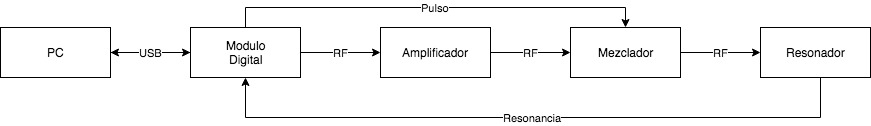
\includegraphics[width=\linewidth]{../figures/d4.jpg}
    \caption{Diagrama de conexiones}
    \label{fig:d4}
\end{figure}
  
%Figure \ref{fig:boat1} shows a boat.

\subsection{Mixer}

Los pulsos de salida y la señal de radiofrecuencia son las entradas del mezclador
donde se convierten en una sola cuando el pulso TTL esta activo en 5 voltios.
Esto permite crear pulsos de estimulacion y relajacion con presicion.

\subsection{Amplificador}


\subsection{Resonador}



\newpage

\section{Visi\'on general del sistema}

Este diagrama respresenta la interacci\'on entre los diferentes elementos de hardware 
y software en una experiencia planificada.

\begin{figure}[!htb].
    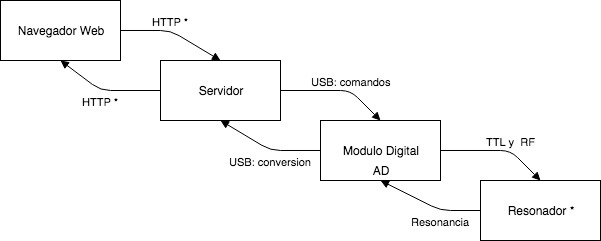
\includegraphics[width=\linewidth]{../figures/d5.jpg}
    \caption{Visi\'on General del sistema}
    \label{fig:d5}
\end{figure}

\subsection{Navegador web}
El navegador web es la plataforma donde se provee al usuario final la interfaz con el sistema.

\subsection{Servidor}
El servidor provee servicios REST solicitados por la interfaz gr\'afica durante la vida
de la sesi\'on del usuario. Estos servicios hacen llamadas al controlador del M\'odulo
Digital via usb.

\subsection{M\'odulo Digital}
El m\'odulo digital procesa los mensajes del controlador via usb y ejecuta 
el microc\'odigo del mismo para la configuraci\'on y ejecuci\'on de las secuencias de pulsos.

\subsection{Resonador}
El resonador recibe los pulsos provenientes del M\'odulo Digital generando una se\~nal de resonancia
enviada al M\'odulo Digital para su conversi\'on digital.

\newpage
\section{Descripci\'on del m\'odulo digital}

El siguiente diagrama de bloques muestra la configuraci\'on interna 
del aparato junto a sus caracter\'isticas t\'ecnicas.

\begin{figure}[!htb].
    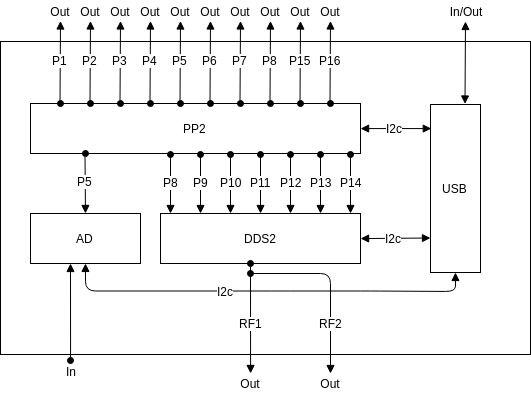
\includegraphics[width=\linewidth]{../figures/d6.jpg}
    \caption{Diagrama de bloques del m\'odulo digital}
    \label{fig:d6}
\end{figure}


\newpage

\section{Subm\'odulo DDS2}

El DDS2 es un generador de se\~nales con un rango de frecuencia de 0 a 120 Mhz.

El usuario puede almacenar hasta 2 frecuencias y un total de 16 fases para 
combinarlos en la ejecuci\'on de un programa.

Tambien hay una relaci\'on entre el PP2 y el DDS2, puesto que este tiene como entrada
los pulsos 8,9,10,11,12,13,14 para su manipulaci\'on externa por aquel durante
la ejecuci\'on de un programa.

\subsection{Configuraci\'on inicial, activaci\'on y desactivaci\'on.}

\begin{table}[ht]
    \centering
    \begin{tabular}{|l|l|l|l|l|l|l|l|l|l|l|}
    \hline
    Direcci\'on  &B7 & B6 & B5 & B4& B3 & B2& B1 & B0 &Hex\\
    \hline
    1D  &0 & 0 & 0 & 1& 1 & 1& 1 & 1 &0x17\\
    \hline
    1E  &0 & 1 & 0 & 0& 0 & 1& 0 & 0 &0x44\\
    \hline
    1F  &0 & 0 & 0 & 0& 0 & 0& 1 & 0 & 0x02\\
    \hline
    20  &0 & 0 & 0 & 0 & 0 & 0& 0 & 0&0x00 \\
    \hline
    \end{tabular}
    \caption{\label{tab:dds2_config_inicial}Reset}
    \end{table}

    \begin{table}[ht]
    \centering
    \begin{tabular}{|l|l|l|l|l|l|l|l|l|l|l|}
    \hline
    Direccion  &B7 & B6 & B5 & B4& B3 & B2& B1 & B0 &Hex\\
    \hline
    1D  &0 & 0 & 0 & 1& 0 & 0& 0 & 0 &0x10\\
    \hline
    1E  &0 & 1 & 0 & 0& 0 & 1& 0 & 0 &0x44\\
    \hline
    1F  &0 & 0 & 0 & 0& 0 & 0& 1 & 0 & 0x02\\
    \hline
    20  &0 & 0 & 0 & 0 & 0 & 0& 0 & 0&0x00 \\
    \hline
    \end{tabular}
    \caption{\label{tab:dds2_activate}Activaci\'on}
    \end{table}
    
    \begin{table}[ht]
    \centering
    \begin{tabular}{|l|l|l|l|l|l|l|l|l|l|l|}
    \hline
    Direcci\'on  &B7 & B6 & B5 & B4& B3 & B2& B1 & B0 &Hex\\
    \hline
    1D  &0 & 0 & 0 & 1& 1 & 1& 1 & 1 &0x17\\
    \hline
    1E  &0 & 1 & 0 & 0& 0 & 1& 0 & 0 &0x44\\
    \hline
    1F  &0 & 0 & 0 & 0& 0 & 0& 1 & 0 & 0x02\\
    \hline
    20  &0 & 0 & 0 & 0 & 0 & 0& 0 & 0&0x00 \\
    \hline
    \end{tabular}
    \caption{\label{tab:dds2_deactivate}Desactivaci\'on}
    \end{table}
\newpage
\subsection{Registros del DDS2}
\begin{table}[ht]
    \centering
    \begin{tabular}{|l|l|l|l|}
    \hline
    Direcci\'on  & Descripci\'on             & Modo      \\
    \hline
    0x70       & direccionamiento        & Escritura \\
    \hline
    0x71       & modo                    & Escritura \\
    \hline
    0x72       & reset                   & Escritura \\
    \hline
    0x73       & test                    & Lectura   \\
    \hline
    0x74       & se\~nal de escritura      & Escritura \\
    \hline
    0x75       & direccionamiento        & Escritura \\
    \hline
    0x76       & se\~nal de transferencia  & Escritura \\
    \hline
    0x77       & test                    & Lectura   \\
    \hline
    0x78       & se\~nal de escritura      & Escritura \\
    \hline
\end{tabular}
\caption{\label{tab:registros_internos_dds2}Resgistros internos del DDS2.}
\end{table}


\subsection{Fases}

El DDS2 tiene disponible 32 posiciones de 8 bits para el almacenamiento de fases
y cuenta con un bus de 8 bits.

El MSB de una fase debe almacenarse siempre en una direcci\'on par de la RAM, luego
el LSB de la misma en el valor impar siguiente contiguo.

La fase es un valor de 14 bits, por lo que los 2 bits restantes del MSB son descartados.

Antes de almacenar el valor entero de la fase F debemos convertirlo a su equivalente
en unidades de 45 de la siguiente manera:
\begin{gather}
        F_h \in \mathbb{N} \\
        F_l \in \mathbb{N} \\
        F \in \mathbb{N} \\
        F_h = (45 * F) / 256 \\          
        F_l = (45 * F) - (F_h * 256)
\end{gather}

\begin{table}[ht]
    \centering
    \begin{tabular}{|l|l|l|}
    \hline
    direcciones de ram disponibles           & Modo \\
    \hline
    0x00 0x02 0x04 0x06 0x08 0x0A 0x0C 0x0E  & 0x02 \\
    \hline
    0x10 0x12 0x14 0x016 0x18 0x1A 0x1C 0x1E & 0x02 \\
    \hline
\end{tabular}
\caption{\label{tab:tableTestCases}Direcciones de Fase.}
\end{table}

\subsubsection{Algoritmo base de almacenamiento de fases}
\begin{algorithm}[H]
    \caption{almacenamiento de una fase en direccion 0x00}\label{algo_phases}
    \begin{algorithmic}[1]
    \Procedure{SavePhase}{F}
    \State // {MSB y LSB de valor de fase}
    \State $F_h = (45 * F) / 256$         
    \State $F_l = (45 * F) - (F_h * 256)$
    \State // {direcciones contiguas}
    \State $dir_h \gets 0x00$
    \State $dir_l \gets dir_h + 1$
    \State // {Modo carga de fases}
    \State $write(0x71, 0x02)$
    \State // {MSB}
    \State $write(0x70, dir_h)$ 
    \State $write(0x74, f_h)$
    \State // {LSB}
    \State $write(0x70, dir_l)$
    \State $write(0x74, f_l)$
    \State // {Modo PC}
    \State $write(0x71, 0x00)$
    \EndProcedure
    \end{algorithmic}
\end{algorithm}

\subsubsection{direccionamiento de fases}
Los 16 valores de fase son direccionados con 4 pulsos correspondientes a los 
pulsos 11,12,13,14. Con el pulso 9 se activa la carga de fases y con el pulso 10
se transfiere la fase direccionada al registro de trabajo.
El tiempo entre el pulso 9 y 10 debe ser menor a 100 nanosegundos.

\subsection{Frecuencias}

El DDS2 tiene disponible 12 registros internos de frecuencia, cada frecuencia ocupa 6 registros, 
por lo tanto se pueden almacenar 2 frecuencias.

Las frecuencias disponibles van de 0 a 120 Mhz y el valor que se almacena en los registros
en representaci\'on se obtiene con la siguiente c\'alculo:
\noindent
\begin{gather}
    clock = 2 \times 10^{6} \\
    frec \in \mathbb{N} \land 0 < frec < clock\\
    valor = frec \times (2^{48} -1 ) / clock
\end{gather}

\begin{table}[ht]
    \centering
    \begin{tabular}{|l|l|l|l|}
    \hline
    Nro. Frecuencia    & Registros       & Modo \\
    \hline
     1 & 0x04 0x05 0x06 0x07 0x08 0x09   & 0x00 \\
    \hline
     2 & 0x0A 0x0B 0x0C 0x0D 0x0E 0x0F   & 0x00 \\
    \hline
\end{tabular}
\caption{\label{tab:registros_frec}Registros de Frecuencia.}
\end{table}

\subsubsection{Algoritmo base de almacenamiento de frecuencias}
\begin{algorithm}[H]
    \caption{almacenamiento de una frecuecia de trabajo 1.}\label{algo_frec}
    \begin{algorithmic}[1]
    \Procedure{SaveFrequency}{F}
    \State // {Conversi\'on de la frecuencia deseada al valor}
    \State $clock \gets 2 \times 10^{6}$
    \State $value = frec \times (2^{48} -1 ) / clock $
    \State // {Modo PC}
    \State $write(0x71, 0x00)$
    \State // {primero MSB hasta LSB}
    \State // {Byte 5}
    \State $write(0x75, 0x04)$ 
    \State $write(0x78, value_5)$
    \State // {Byte 4}
    \State $write(0x75, 0x05)$ 
    \State $write(0x78, value_4)$
    \State // {Byte 3}
    \State $write(0x75, 0x06)$ 
    \State $write(0x78, value_3)$
    \State // {Byte 2}
    \State $write(0x75, 0x07)$ 
    \State $write(0x78, value_2)$
    \State // {Byte 1}
    \State $write(0x75, 0x08)$ 
    \State $write(0x78, value_1)$
    \State // {Byte 0}
    \State $write(0x75, 0x09)$ 
    \State $write(0x78, value_0)$
    \State // {Actualizaci\'on registro de trabajo}
    \State $write(0x76, 0x00)$
    \EndProcedure
    \end{algorithmic}
\end{algorithm}

\subsubsection{direccionamiento de frecuencias}
Se admiten hasta 2 frecuencias de trabajo, se seleccionan con el pulso 8.

\newpage

\section{Submodulo AD}

El submodulo conversor analogico digital (AD) tiene 2 canales de adquisicion,
con una resolucion de 12 bits por canal, una frecuencia de muestreo maxima de 10 Mhz 
y capacidad de almacenamiento en bloques de 1KB,2KB,4KB,8KB,16KB,32KB,64KB,128KB.

\begin{table}[ht]
    \centering
    \begin{tabular}{|l|l|l|}
    \hline
     Direccion   & Descripcion       & modo\\
    \hline
     0x0B        & comando y control & lectura/escritura\\ 
    \hline
     0x0C        & muestreo          & escritura\\
     \hline
     0x08        & canal B           &lectura   \\
     \hline
     0x09        & canal AB          &lectura   \\
     \hline
     0x0A        & canal A           &lectura   \\
     \hline
\end{tabular}
\caption{\label{tab:registros_ad} Registros del AD}
\end{table}

\subsection{Registro de comando}
\begin{table}[ht]
    \centering
    \begin{tabular}{|l|l|l|}
    \hline
    Bit    & Descripcion \\
    \hline
     0 & modo\\ 
    \hline
     1 & modo\\
     \hline
     2 & - \\
     \hline
     3 & - \\
     \hline
     4 & bloque \\
     \hline
     5 & bloque \\
     \hline
     6 & bloque \\
     \hline
     7 & reset \\
     \hline
\end{tabular}
\caption{\label{tab:registros_ad_cmd}Registro de comando.}
\end{table}

\subsection{Registro de datos}

\begin{table}[ht]
    \centering
    \begin{tabular}{|l|l|l|}
    \hline
    Direccion & Descripcion \\
    \hline
     0x08 & canal B\\ 
    \hline
     0x09 & canal AB\\
     \hline
     0x0A & canal A\\
     \hline
\end{tabular}
\caption{\label{tab:registros_ad_datos}Registros de datos.}
\end{table}


\subsection{Configuracion de un ciclo de adquisicion}

Un ciclo de adquisicion requiere la configuracion del intervalo de muestreo
de acuerdo a la siguiente formula:
\begin{gather}
period = 100 ns\\
interval \in \mathbb{N} \land 0 < interval < 25500\\
n = interval / period\\
delta  = 255 - n\\
\end{gather}

\subsubsection{Configuracion bloque de 1K muestreo 1 micro seg}

\begin{algorithm}
    \caption{Configuracion 1K 1micro}\label{algo_ad_conf}
    \begin{algorithmic}[1]
    \Procedure{Setup}{}
    \State
    \State $config \gets 0x00$
    \State $config \gets config \lor 0x02$
    \State $config \gets config \lor 0x80$
    \State $config \gets config \land 0xFE$
    \State $write(0x0B, config)$
    \State
    \State $config \gets 0x00$
    \State $config \gets config \lor 0x02$
    \State $config \gets config \land 0x7F$
    \State $config \gets config \lor 0x01$
    \State $write(0x0B, config)$
    \State
    \State $samples= 1000 / 100$
    \State $delta = 255 - samples$
    \State $write(0x0C, delta)$

    \EndProcedure
    \end{algorithmic}
    \end{algorithm}
    \newpage
\subsection{Extraccion de los datos de la memoria interna}

El bus de datos de la memoria del AD es de 8 bits y las muestras de 12 bits,
siendo necesarias 3 lecturas de 8 bits y una operacion de particion para
obtener la muestra final de los canales A y B.

\begin{figure}[!htb].
    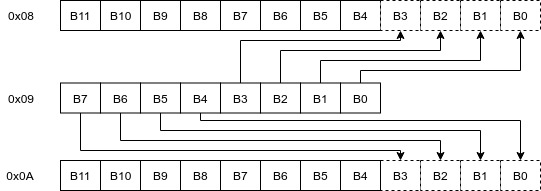
\includegraphics[width=\linewidth]{../figures/d8.jpg}
    \caption{Buffers del submodulo AD}
    \label{fig:d8}
\end{figure}

Para la extraccion de los datos es necesaria esta serie de pasos:

\begin{itemize}
    \item modo PC, deshabilitada la adquisicion y reset contador de direcciones
    \item modo PC, deshabilitada la adquisicion y contador de direcciones en modo normal
    \item lectura del registro 0x08 del canal B
    \item modo PC, deshabilitada la adquisicion y reset contador de direcciones
    \item modo PC, deshabilitada la adquisicion y contador de direcciones en modo normal
    \item lectura del registro 0x0A del canal A
    \item modo PC, deshabilitada la adquisicion y reset contador de direcciones
    \item modo PC, deshabilitada la adquisicion y contador de direcciones en modo normal
    \item lectura del registro 0x09 con nibles del canal A y B.
    \item armado de los datos de los respectivos canales.
\end{itemize}

\begin{algorithm}
    \caption{Extraccion de datos}\label{algo_ad_data}
    \begin{algorithmic}[1]
    \Procedure{Setup}{}
   
    \State $config \gets 0x00$
    \State $config \gets config \lor 0x02$
    \State $config \gets config \lor 0x80$
    \State $config \gets config \land 0xFE$
    \State $write(0x0B, config)$
    \State $config \gets 0x00$
    \State $config \gets config \lor 0x02$
    \State $config \gets config \land 0x7F$
    \State $config \gets config \land 0xFE$
    \State $write(0x0B, config)$
    \State $A \gets read(0x08)$
    \State
    \State $config \gets 0x00$
    \State $config \gets config \lor 0x02$
    \State $config \gets config \lor 0x80$
    \State $config \gets config \land 0xFE$
    \State $write(0x0B, config)$
    \State $config \gets 0x00$
    \State $config \gets config \lor 0x02$
    \State $config \gets config \land 0x7F$
    \State $config \gets config \land 0xFE$
    \State $write(0x0B, config)$
    \State $B \gets read(0x0A)$
    \State
    \State $config \gets 0x00$
    \State $config \gets config \lor 0x02$
    \State $config \gets config \lor 0x80$
    \State $config \gets config \land 0xFE$
    \State $write(0x0B, config)$
    \State $config \gets 0x00$
    \State $config \gets config \lor 0x02$
    \State $config \gets config \land 0x7F$
    \State $config \gets config \land 0xFE$
    \State $write(0x0B, config)$
    \State $AB \gets read(0x09)$
    \State
    \State $sample\_A \gets join\_buffers(A, AB)$
    \State $sample\_B \gets join\_buffers(B, AB)$

    \EndProcedure
    \end{algorithmic}
    \end{algorithm}



\newpage

\section{Submodulo PP2}
\section{Submodulo USB}
\newpage
\section{Definici\'on de un experimento}

Para representar la definici\'on de un experimento se eligi\'o notaci\'on JSON, 
por el soporte built-in por parte de los lenguajes usados para desarrollar el sistema, 
Python y Javascript, tambi\'en por la implementaci\'on de servicios REST necesarios 
en el \textit{Servidor}\cite{json_standar}.
Haciendo uso de aritm\'etica podemos deducir que la representaci\'on de un experimento en JSON
es liviana puesto que el n\'umero de instrucciones de un programa \(P\) ser\'a de \(N < 512 \) 
y para un archivo de texto de 512 l\'ineas y 80 columnas de caracteres de 1 Byte 
tiene un peso aproximado de 327.68 Kilobytes.
La validaci\'on del esquema JSON de un experimento, es llevada a cabo por un m\'odulo programado
dentro del sistema para tal fin.
Cabe destacar que los tipos de datos presentes en la especificaci\'on de un experimento son
soportados sin p\'erdida de precisi\'on por parte de la notaci\'on JSON.\cite{json_ref}

\lstset{
    string=[s]{"}{"},
    stringstyle=\color{blue},
    comment=[l]{:},
    commentstyle=\color{black},
}

\begin{lstlisting}
{
  "cpoints": [
    {
      "lsb": "00000011",
      "freq_unit": "hz",
      "t_unit": "ns",
      "type": "C",
      "msb": "00000011",
      "time": "10",
      "phase": "0",
      "freq": "100",
      "data": "0",
      "id": 1535931832181
    }
  ],
  "settings": {
    "a_times": "3",
    "a_name": "exp 1",
    "a_channel": "3",
    "a_description": "descr exp 1",
    "a_freq": "100",
    "a_msb": "00000000",
    "a_freq_unit": "hz",
    "a_ts_unit": "ns",
    "a_lsb": "00000000",
    "a_ts": "100",
    "a_bloq": "1",
    "a_phase": "0"
  },
  "execute": true
}
\end{lstlisting}

\newpage


\section{Algoritmo de traduccion de experimentos}

Esta seccion describe como un experimento es traducido a instrucciones que el PP2 pueda almacenar y ejcutar.

Como mencionamos en el capitulo XX un programa almacenable y ejecutable por el PP2 es una secuencia de 
instrucciones I1 .. IN con N no mayor a K, donde K esta relacionado al limite de memoria del mismo es de XX MB.

Las instrucciones disponibles son:

*continue
*loop
*retl
*fin

No todos los programas escritos con estas instrucciones son admitidos como validos para el PP2, 
por esto tenemos las siguientes reglas que deben cumplir los programas ejecutables por el PP2.

Regla 1:
la instruccion fin siempre es la ultima instruccion.

Regla 2:
la intruccion fin aparece solo una vez.

Regla 3:
la intruccion fin siempre esta presente.

Regla 4:
un bloque siempre inicia con instruccion loop y finaliza con retl

Regla 5:
puede haber hasta 3 loops dentro de un loop

Estas reglas definen el siguiente automata:



Resultando en el siguiente algoritmo base: 


traslate(P, L, S)

    ins = next(P)

    if ins = Continue:
        S.append(ins)

    if ins = Retl:
        if(L!=0):
            S.append(ins)
            L--
        else:
            ret Error

    if ins = Loop:
        if(L<4):
            S.append(ins)
            L++
        else:
            ret Error
    
    ret S
\section{Ejecuci\'on de un experimento}

Un modo de capturar fallos es simular la ejecuci\'on de un experimento,
evitando la interacci\'on via usb, con el m\'odulo digital.
En modo simulado el experimento se ejecuta en un entorno limitado con el objetivo de
detectar tres situaciones no deseadas:

\begin{itemize}
\item Una exepci\'on de software no capturada.
\item Par\'ametros fuera de rango para alguno de los subm\'odulos.
\item Un error en la traducci\'on del experimento a un programa ejecutable en el PP2.
\end{itemize}

Un experimento simulado se ejecuta el hilo principal, puesto que 
la demora es baja. De manera alternativa el modo simulado puede verse tambi\'en como un 
test de integraci\'on entre las unidades de software desarrolladas.
Si el experimento simulado tiene \'exito entonces se procede con la ejecuci\'on efectiva
del experimento que se desprende del hilo princial y en el cual debemos tener 
algunos detalles en cuenta:

\begin{itemize}
    \item Puede durar horas.
    \item Puede ser interrumpido por el usuario en cualquier momento.
    \item Debe estar sincronizado con la base de datos.
\end{itemize}

El siguiente diagrama muestra el flujo de ejecuci\'on de un experimento simulado y no simulado.

\newpage
\section{Hilo de ejecuci\'on de un experimento}

La duraci\'on de un experimento puede ser de horas, esta caracter\'istica involucra tres problematicas
a resolver:

\begin{itemize}
    \item Evitar time-out del lado del cliente web.
    \item Desacoplar la atenci\'on de una petici\'on HTTP de usuario de la ejecuci\'on de un experimento.
    \item Lograr una experiencia de usuario agradable en lo que respecta a performance.
\end{itemize}

Modelando el proceso de ejecuci\'on con un hilo separado del principal es una soluci\'on
v\'alida para resolver el problema y teniendo en cuenta los siguientes:

\begin{itemize}
    \item Seguimiento del estado del hilo.
    \item Control sobre el numero de hilos creados.
    \item Gesti\'on de los datos durante la ejecuci\'on del hilo.
\end{itemize}

\begin{figure}[!htb].
    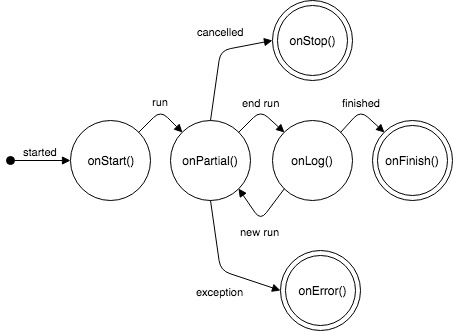
\includegraphics[width=\linewidth]{../figures/d14.jpg}
    \caption{Estados de un hilo de experiemento.}
    \label{fig:d14}
\end{figure}

\newpage
\section{Diagrama de flujo de ejecucion de un experimento}

El siguiente diagrama describe la ejecucion de un experimento dry-run y main-run
\newpage
\section{Requisitos del sistema}

Podemos ver los requerimientos en generales


* permitir a mas de un usuario utilizar el sistema
* permitir a usuarios la gestion de experimentos
* modelar un experimento y su ejecucion
* proveer acceso remoto al sistema

De estos requerimientos se desprenden los siguientes especificos:

* el usuario tiene una sesion asignada al ingreso del sistema y revocada a la salida del mismo.
* varios usuarios pueden acceder al sistema al mismo tiempo


* el usuario puede ver si hay un experimento en ejecucion y el detalle del mismo
* el usuario tiene un espacio de trabajo donde puede crear/ver/actualizar/eliminar sus experimentos
* el usuario puede cancelar el experimento en ejecucion
* el usuario puede solicitar un reporte parcial de un experimento en ejecucion
* el usuario puede solicitar el reporte final de un experimento finalizada la ejecucion
* el usuario puede verificar el estado de un experimento:
* el usuario es notificado antes de la ejecucion de un experimento cuando:
    * salida voluntaria por error:
        * no es una secuencia ejecutable por el PP2
        * ya existe algun experimento ejecutandose
        * algun parametro de configuracion es invalido en algun submodulo PP2, DDS2, AD, USB
        * fallo en conexion via USB
    * salida involuntaria por error:
        * hubo alguna excepcion de sistema no controlada
        * no se pudo establecer conexion con el servidor
        * un experimento finalizado no actualizo su estado impidiendo la ejecucion de solcitido

* un experimento tiene una secuencia definidida con sus parametros
* un experimento tiene una marca de tiempo de creacion/actualizacion
* un experimento eliminado no es recuperable
* un experimento tiene un autor que es el usuario que lo creo
* un experimento tiene estado created cuando esta almacenado en base de datos
* un experimento es solo visible para el usuario que lo creo
* un experimento tiene un titulo
* un experimento tiene una descripcion
* un experimento no tiene un historial de edicion asociado

* un resultado es el producto de la ejecucion de un experimento
* un resultado es parcial cuando la ejecucion del experimento asociado no finalizo
* un resultado es final cuando la ejecucion del experimento asociado finalizo
* un resultado tiene un unico experimento asociado

* un reporte parcial es el grupo de datos de un resultado parcial
* un reporte final es el grupo de un resultado final
* un reporte contiene:
    * log de la ejecucion
    * datos del AD en formato CSV
    * experimento ejecutado

* el sitema tiene servicios REST para:
    * crear/ver/editar/eliminar experimentos
    * iniciar/cancelar ejecucion de un experimento
    * cancelar la ejecucion de todos los experimentos
    * descargar reportes parciales y finales
    * proveer autenticacion a todos los servicios

* el sistema tiene una interfaz de usuario web
\newpage
\section{Planificacion del desarrollo}


De acuerdo con los requerimientos descriptos en el capitulo XX se propone implementar el sistema
con:

    * Django framework - Pythton 2.7
    * React js - Javascript ECM6
    * Git

Las tecnologias elegidas son ampliamente soportadas por la comunidad de desarrolladores, de codiglo libre y soporte multiplataforma en PC.

Con el objetivo de asegurar que lo primero que se desarrolle cumpla son los requeriminetos asociados 
con el control del Modulo Digital, luego proveer una manipulacion remota y finalmente una interfaz de
usuario para el manejo a traves del navegador web, se organizo el desarrollo de la siguiente manera:

    * Modulo Digital
    * Servidor 
    * Interfaz Grafica Web

El mapeo entre los requerimentos y el orden propuesto genera el siguiente esquema de tareas a realizar.

    * Modulo Digital
        - Configuracion del proyecto y entornos
        - Implementacion control AD 
        - Implementacion control DDS2
        - Implementacion control PP2
        - Implementacion abstraccion Experimento
        - Implementacion de interfaz USB
        - Implementacion de un programa principal
        - Gestion de logs
        - Integracion con Servidor

    * Servidor
        - Configuracion del proyecto y entornos
        - Servicios REST para la edicion de experimentos
        - Servicios REST para control de ejecucion de experimentos
        - Servicios REST para la generacion de reportes
        - Modelado de Base de datos 
        - Configuracion de sesiones
        - Configuracion de acceso a los servicios REST
        - Gestion de logs
        - Integracion con Interfaz WEB
        - Integracion con Modulo Digital
    
    * Interfaz WEB
        - Configuracion de proyecto y entornos
        - Implementacion de transiciones
        - Componente de edicion de experimentos
        - Componente de control de ejecucion de experimentos
        - Componente de login
        - Componente de visualizacion de errores
        - Componente de definicion de experimento
        - Implementacion de control de estados
        - Integracion con Servidor

\section{Planificacion de Testing}

La planificacion de testing del sistema tiene varios enfoques en respuesta a diferentes objetivos:

    * brindar una experiencia predecible y agradable al usuario final
    * lograr una integracion coherente entre modulos
    * aumentar cobertura de requerimientos de usuario y sistema
    * facilitar la comprension del comportamiento esperado del sistema

Por unidad existen las siguientes validaciones:

    Modulo Digital
        
        * entradas de configuracion para el PP2, DDS2 y AD
        * entradas de programa ejecutable por el PP2
        * existencia de conexion via interfaz USB durante la ejecucion de experimentos
        * salidas de señales RF
        * salidas de pulsos TTL
        * input de conversion de datos del AD
        * salida de reportes de los canales A y B.

    Servidor

        * autenticacion obligatoria en los servicios
        * ejecucion secuencial de los experimentos
        * aislamiento de espacio de trabajo de usuarios
        * coherencia en los estados de los experimentos
        * generacion de reportes
        * gestion de procesos de ejecucion de experimentos

    Interfaz de usuario web

        * visualizacion coherente de elementos y estilos
        * tiempos cortos de carga de las vistas
        * visualizacion de alertas de usuario
        * transiciones entre vistas

Dados los diferentes enfoques son necesarias se eligieron las siguientes para probar:

    * Postman para simular comunicacion http con servicios REST
    * Arduino para visualizar los pulsos TTL via Serial Plotter
    * Osciloscopio para medir señales RF generadas en los experimentos.
    * Generador de señales para simular adquisicion de datos del AD.
    * Google Chrome y herramientas para validar estados de la interfaz grafica.
    * Mock del servidor escrito en Flask-Python para simular servicios REST.

    \newpage
\section{Arquitectura del Modulo Digital}
\begin{figure}[!htb].
    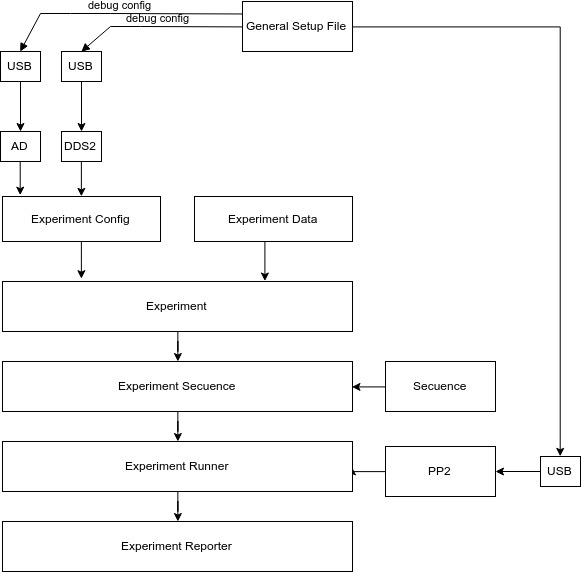
\includegraphics[width=\linewidth]{../figures/d19.jpg}
    \caption{Arquitectura Modulo Digital}
    \label{fig:d19}
\end{figure}
\newpage
\section{Arquitectura del Servidor}
\newpage
\section{Arquitecturra de Interfaz Grafica}
\newpage
\section{Integracion de los submodulos}

La integracion de los modulos del sistema se implementa a diferentes niveles:


Repositorio

Un submodulo git es un repositorio dentro de otro que lo incluye, con su propio historial de cambios. Asi mismo cuando hay un cambio en un submodulo el contenedor lo contemplara siempre y cuando lo agregue al historial de este.
El repositorio afectado por esta metodologia es el del Servidor incluyento al Modulo Digital y a la Interfaz Grafica.

El arbol de directorios del repositorio queda asi:


Codigo:

El servidor provee el ManagerThread para poder interactuar con el Modulo Digital y con el 
modelo de la base de datos segun el estado de la ejecucion del experimento en curso.

Para integrar con la Interfaz grafica lo hace de manera estandar via configuracion del servidor
que provee seguridad y autenticacion de los servicios via CSRF-Token presente en el archivo
principal index.html de la Interfax Grafica.


\section{Analisis de Performance}


Se propone como analisis de performace un experimento con las siguientes caracteristicas:

* 500 promedios
* 2 loops con un pulso cada uno
* bloque de 8K
* 4 fases

Los consumos de CPU - RAM - DISCO
\newpage
\section{Casos de Prueba}

De acuerdo con los enfoques generales y por unidad se dise\~naron los siguientes casos de prueba:

\subsection{M\'odulo Digital}
\begin{itemize}
\item Experimento con configuraci\'on inv\'alida del AD.
\item Experimento con configuraci\'on inv\'alida del DDS2.
\item Experimento con secuencia inv\'alida para el PP2.
\item Experimento con un pulso largo.
\item Experimento con un pulso corto.
\item Experimento con pulsos largos y cortos intercalados.
\item Experimento promedio con un pulso.
\item Experimento promedio con un pulso variable en duraci\'on.
\item Experimento promedio con un pulso variable en fase.
\item Experimento con un pulso dentro de un \textit{loop}.
\item Experimento con un pulso dentro de un \textit{loop} de nivel 4.
\item Experimento con un \textit{retl} sin \textit{loop} asociado.
\item Experimento con un \textit{loop} sin \textit{retl} asociado.
\item Experimento con un \textit{loop} de nivel 5.
\end{itemize}

\subsection{Servidor}
\begin{itemize}
\item Solicitud de servicio sin token de autenticaci\'on.
\item Solicitud de autenticaci\'on con usuario no registrado.
\item Solicitud de autenticaci\'on con usuario registrado pero contrase\~na inv\'alida.
\item Solicitud de fin de sesi\'on.
\item Solicitud de creaci\'on de un experimento.
\item Solicitud de edici\'on de un experimento.
\item Solicitud de edici\'on de un experimento inexistente.
\item Solicitud de edici\'on de un experimento en ejecuci\'on.
\item Solicitud de eliminaci\'on de un experimento.
\item Solicitud de eliminaci\'on de un experimento inexistente.
\item Solicitud de eliminaci\'on de un experimento en ejecuci\'on.
\item Solicitud de ejecuci\'on de un experimento habiendo uno en ejecuci\'on.
\item Solicitud de ejecuci\'on de un experimento inexistente.
\item Solicitud de ejecuci\'on de un experimento.
\item Solicitud de cancelaci\'on de una ejecuci\'on en curso.
\item Solicitud de reporte durante la ejecuci\'on.
\item Solicitud de reporte finalizada la ejecuci\'on.
\item Solicitud de reporte de un experimento que nunca se ejecuto.
\item Solicitud de reporte de una ejecuci\'on cancelada.
\item Solicitud de reporte de una ejecuci\'on fallida.
\end{itemize}

\subsection{Interfaz Grafica}
\begin{itemize}
\item Ingreso al sitio con usuario y contrase\~na v\'alidos.
\item Ingreso al sitio con usuario ó contrase\~na inv\'alidos.
\item Salida del sitio con bot\'on login.

\item Crear un experimento con sus variantes.

\item Visualizaci\'on de lista de experimentos creados.
\item Filtrado de lista de experimentos creados.

\item Ver un experimento seleccionado de la lista
\item Edici\'on de un experimento seleccionado de la lista
\item Eliminaci\'on de un experimento seleccionado de la lista
\item Ejecuci\'on de un experimento seleccionado de la lista

\item Visualizaci\'on de lista de resultados
\item Visualicaci\'on de detalles de un resultado
\item Visualizaci\'on de men\'u de gestion de experimentos
\item Visualizaci\'on de men\'u de gestion de resultados
\item Visualizaci\'on de men\'u de navegaci\'on
\item Visualizaci\'on de alertas
\end{itemize}
\newpage
\section{Errores conocidos}

\begin{itemize}
    \item si el sistema es interrumpido por un apagado imprevisto durante una ejecucion 
        es posible que un estado sea inconcistente

    \item en vista edicion hacer click en boton "guardar y ejecutar" demora 5 segundos la transicion a 
        vista de resultados

    \item las alertas deben ser cerradas para obtener nuevas si las hubiese

    \item soporte parcial a diferentes tamaños de pantalla
\end{itemize}
\newpage
\section{Limitaciones del sistema}

Existen limitaciones de diversos tipos:

\begin{itemize}
    \item Plataforma
    \begin{itemize}
    \item Driver y DLL USB disponible para windows \'unicamente.
    \item Administraci\'on de filesystem restrictiva. 
    \item Soporte librer\'ias de matem\'atica y gr\'aficos limitada.
    \item Celery y RabbitMQ no son soportados completamente.
    \end{itemize}
    \item M\'odulo Digital
    \begin{itemize}
        \item Requiere la implementaci\'on de un manager para su utilizaci\'on
    \end{itemize}
    \item Server
    \begin{itemize}
        \item Gesti\'on del proceso del servidor requiere un sysadmin siempre.
        \item Gesti\'on de usuarios es manual via interfaz Django, no autoadministrable.
        \item Seguimiento de recursos de sistema es manual, no hay pol\'itica de balance de carga.
    \end{itemize}
    \item Interfaz Gr\'afica
    \begin{itemize} 
        \item JQuery no es soportado seg\'un directrices de ReactJs.
    \end{itemize}
\end{itemize}
\newpage

\section{Mejoras a futuro}

\begin{itemize}

\item Modulo digital
    \begin{itemize}
    \item interfaces de servicio
    \item independencia como programa de consola
    \item test automaticos
    \item integracion continua
    \end{itemize}
\item Server
    \begin{itemize}
    \item cola de experimentos
    \item soporte a otros Modulos Digitales u Aparatos
    \item post-procesado de datos en tiempo real
    \item test automaticos
    \item integracion continua
    \end{itemize}
\item Interfaz Grafica
    \begin{itemize}
    \item soporte a telefonos moviles
    \item visualizacion de graficos
    \item tests automaticos
    \item vista de manipulacion de resultados
    \item vista de gestion de perfil
    \item tests automaticos
    \item integracion continua
    \end{itemize}
\end{itemize}
\newpage
\section{M\'etricas de desarrollo}

Se presentan algunas m\'etricas tales como total de l\'ineas de c\'odigo y commits de los proyectos
obtenidos con los comandos:
\begin{lstlisting}[language=bash]
    $ git ls-files | xargs wc -l , $ git log --oneline | wc -l y $cloc
\end{lstlisting}
respectivamente.
  
\begin{itemize}
\item Módulo Digital (57 Commits)
\begin{lstlisting}[language=bash]
        2 .gitignore
        674 LICENSE
        133 Microchip/mpusbapi.dll
         84 Microchip/mpusbapi.h
          0 __init__.py
         50 dry_run.py
         55 main.py
         49 main_logger.py
        131 source/Usb.py
          0 source/__init__.py
        193 source/ad.py
        228 source/dds2.py
         27 source/experiment2.py
         17 source/experiment_config.py
         53 source/experiment_data.py
         47 source/experiment_reporter.py
         23 source/experiment_runner.py
        271 source/experiment_scanner.py
        125 source/experiment_secuence.py
        108 source/pp2.py
         59 source/secuence.py
          7 source/setup.py
        263 tests.py
       2599 total
    \end{lstlisting}

\item Interfaz Gr\'afica (27 Commits)
\begin{lstlisting}[language=bash]
        24 .gitignore
        2164 README.md
          24 package.json
          12 public/favicon.ico
          45 public/index.html
          15 public/manifest.json
          35 src/crear_experimento/action_panel/index.js
          34 src/crear_experimento/experiment_admin/index.js
          43 src/crear_experimento/experiment_view/index.css
          33 src/crear_experimento/experiment_view/index.js
         142 src/crear_experimento/experiment_view/modal_generic.js
          82 src/crear_experimento/general_settings/index.js
         146 src/crear_experimento/index.js
          39 src/editar_experimento/action_panel/index.js
          33 src/editar_experimento/experiment_admin/index.js
          43 src/editar_experimento/experiment_view/index.css
          34 src/editar_experimento/experiment_view/index.js
         142 src/editar_experimento/experiment_view/modal_generic.js
          82 src/editar_experimento/general_settings/index.js
         194 src/editar_experimento/index.js
           5 src/index.css
         160 src/index.js
          48 src/intermediate_server/data.js
         150 src/lista_de_experimentos/action_panel/index.js
          44 src/lista_de_experimentos/action_panel/view.js
          42 src/lista_de_experimentos/index.js
          82 src/lista_de_experimentos/table_experiments/index.js
           7 src/logo.svg
          23 src/monitor_de_estado/index.js
           4 src/notification_area/notification.css
          27 src/notification_area/notification.js
          13 src/panel_general/index.css
         107 src/panel_general/index.js
           7 src/panel_general/logo.svg
          10 src/procesamiento_de_datos/index.js
         108 src/registerServiceWorker.js
         139 src/resultado_de_experimentos/action_panel/index.js
          44 src/resultado_de_experimentos/action_panel/view.js
          42 src/resultado_de_experimentos/index.js
          82 src/resultado_de_experimentos/table_experiments/index.js
          64 src/sesion_de_inicio/index.js
          39 src/ver_experimento/action_panel/index.js
          33 src/ver_experimento/experiment_admin/index.js
          43 src/ver_experimento/experiment_view/index.css
          34 src/ver_experimento/experiment_view/index.js
         140 src/ver_experimento/experiment_view/modal_generic.js
          82 src/ver_experimento/general_settings/index.js
         193 src/ver_experimento/index.js
          39 src/ver_resultado/action_panel/index.js
          33 src/ver_resultado/experiment_admin/index.js
          43 src/ver_resultado/experiment_view/index.css
          34 src/ver_resultado/experiment_view/index.js
         140 src/ver_resultado/experiment_view/modal_generic.js
          82 src/ver_resultado/general_settings/index.js
         193 src/ver_resultado/index.js
          74 src/vista_parcial/index.js
        5776 total
    \end{lstlisting}
    
\item Servidor (33 commits):
    \begin{lstlisting}[language=bash]
       0 experiments/__init__.py
       6 experiments/admin.py
       8 experiments/apps.py
      49 experiments/experiment.py
      45 experiments/manager_thread.py
       0 experiments/migrations/__init__.py
      34 experiments/models.py
     195 experiments/result.py
     102 experiments/result_manager_thread.py
       6 experiments/tests.py
      13 experiments/urls.py
     139 experiments/views.py
       0 login/__init__.py
       6 login/admin.py
       8 login/apps.py
       0 login/migrations/__init__.py
       6 login/models.py
       6 login/tests.py
       8 login/urls.py
      28 login/views.py
      22 manage.py
     853 total
    \end{lstlisting}
\end{itemize}
\newpage

A continuaci\'on las m\'etricas provistas por el comando \enquote{cloc} sobre el
repositorio del \textit{Servidor} el cual contiene por integraci\'on al \textit{M\'odulo Digital}
y a la \textit{Interfaz Gr\'afica}.

\begin{lstlisting}[language=bash]
  98 text files.
  81 unique files.                              
  33 files ignored.

github.com/AlDanial/cloc v 1.74  T=0.46 s (162.3 files/s, 16302.6 lines/s)
---------------------------------------------------------------------
Language         files          blank        comment           code
---------------------------------------------------------------------
JavaScript         30            302             54           2226
Python             35            460            234           1860
Markdown           2            676              0           1490
CSS                4              8              0             57
JSON               2              0              0             39
C/C++ Header       1             15             38             31
HTML               1              3             21             21
---------------------------------------------------------------------
SUM:               75           1464            347           5724
---------------------------------------------------------------------
\end{lstlisting}
\newpage
\begin{thebibliography}{9}
    \bibitem{json_ref} 
    \href{https://stackoverflow.com/questions/35709595/why-would-you-use-a-string-in-json-to-represent-a-decimal-number}{JSON notation -https://stackoverflow.com/questions/35709595/why-would-you-use-a-string-in-json-to-represent-a-decimal-number}

    \bibitem{json_standar} 
    \href{https://www.json.org}{Introducing JSON - https://www.json.org}

    \bibitem{django_tutorial} 
    \href{https://docs.djangoproject.com/en/1.11/intro/tutorial01/}{Writing your first Django app - https://docs.djangoproject.com/en/1.11/intro/tutorial01/}

    \bibitem{django_csrf} 
    \href{https://docs.djangoproject.com/en/1.11/ref/csrf/}{Cross Site Request Forgery protection - https://docs.djangoproject.com/en/1.11/ref/csrf/}

    \bibitem{django_cookie} 
    \href{https://docs.djangoproject.com/en/1.11/topics/http/sessions/#cookie-session-backend}{Using cookie-based sessions - https://docs.djangoproject.com/en/1.11/topics/http/sessions/\#cookie-session-backend}

    \bibitem{create_react_app} 
    \href{https://github.com/facebook/create-react-app}{Create React App - https://github.com/facebook/create-react-app}

    \bibitem{react_jquery} 
    \href{https://reactjs.org/docs/integrating-with-other-libraries.html#integrating-with-dom-manipulation-plugins}{ReactJS JQuery Integration - https://reactjs.org/docs/integrating-with-other-libraries.html\#integrating-with-dom-manipulation-plugins}

    \bibitem{git_submodules} 
    \href{https://gist.github.com/gitaarik/8735255}{Git Submodules basic explanation - https://gist.github.com/gitaarik/8735255}

    \bibitem{react_components} 
    \href{https://reactjs.org/docs/components-and-props.html}{Components and Props - https://reactjs.org/docs/components-and-props.html}

    \bibitem{react_state} 
    \href{https://reactjs.org/docs/state-and-lifecycle.html}{State and Lifecycle - https://reactjs.org/docs/state-and-lifecycle.html}

    \bibitem{react_lifting} 
    \href{https://reactjs.org/docs/lifting-state-up.html}{Lifting State Up - https://reactjs.org/docs/lifting-state-up.html}
    
    \bibitem{react_thinking} 
    \href{https://reactjs.org/docs/thinking-in-react.html}{Thinking in React - https://reactjs.org/docs/thinking-in-react.html}
    
    \bibitem{react_router} 
    \href{https://github.com/ReactTraining/react-router}{React Router DOM - https://github.com/ReactTraining/react-router}

    \bibitem{axios} 
    \href{https://github.com/axios/axios}{AxiosJS - https://github.com/axios/axios}

    \bibitem{github} 
    \href{https://github.com}{GitHub Home - https://github.com}

    \bibitem{celery} 
    \href{http://docs.celeryproject.org/en/latest/faq.html#does-celery-support-windows}
    {Does Celery support Windows? - http://docs.celeryproject.org/en/latest/faq.html\#does-celery-support-windows}

\end{thebibliography}
\end{document}